\documentclass{article}
\usepackage{hyperref}

\usepackage[margin = 1in]{geometry}
\usepackage{listings}
\usepackage{mathtools}
\usepackage{apacite}
\usepackage{graphicx} \graphicspath{ {./Images/} }
\usepackage{blindtext}
\usepackage{titling}
\usepackage{setspace} \doublespacing
\usepackage{wrapfig} 
\setlength\parindent{24pt}
\renewcommand\maketitlehooka{\null\mbox{}\vfill}
\renewcommand\maketitlehookd{\vfill\null}

\usepackage{listings}
\usepackage{xcolor}

\definecolor{codegreen}{rgb}{0,0.6,0}
\definecolor{codegray}{rgb}{0.5,0.5,0.5}
\definecolor{codepurple}{rgb}{0.58,0,0.82}
\definecolor{backcolour}{rgb}{0.76, 0.76, 0.76}

\lstdefinestyle{mystyle}{
    backgroundcolor=\color{backcolour},   
    commentstyle=\color{codegreen},
    keywordstyle=\color{magenta},
    numberstyle=\tiny\color{codegray},
    stringstyle=\color{codepurple},
    basicstyle=\ttfamily\footnotesize,
    breakatwhitespace=false,         
    breaklines=true,                 
    captionpos=b,                    
    keepspaces=true,                 
    numbers=left,                    
    numbersep=5pt,                  
    showspaces=false,                
    showstringspaces=false,
    showtabs=false,                  
    tabsize=2
}

\lstset{style=mystyle}


\title{Use of Spiking Neural Networks for Object Detection}
\author{Arslan Salikhov \\
	\and 
	Erik Caceros \\
	\and
	Brandon Lam \\
	}
\date{\today}



\begin{document}

\begin{titlingpage}
\maketitle

\end{titlingpage}


\tableofcontents
\newpage

\section{Introduction}

Use of Deep Neural Network, commonly referred to as
\emph{deep learning} spiked in recent years and has been popular
as a tool for impressive advancements in the field of 
\emph{Artificial Intelligence (AI)}.
The goal of this project was to attempt and recreate a spiking neural network that is capable of object detection, particularly classification and localization. As described, our program was built on Deep Neural Networks, spiking neurons, and convolutional network frameworks, which we find interesting and important. Despite the inability to complete the product we nonetheless met our ultimate goal, to learn more about computational neuroscience. Moreover, our attempt at an object detecting, spiking neural network provided a comprehensive learning experience for all members, regardless of prior knowledge on the subject. 

\subsection{Neural Networks}

% \subsection{Deep Neural Networks}

A Deep Neural Network, DNN, is a machine learning algorithm that tries to mimic how the brain processes information. The reason why DNNs are called deep is due to the networks having more than two hidden layers. The increased number of hidden layers enables DNNs to complete more complicated tasks compared to their shallow counterparts. However, increasing the number of hidden layers increases the training time in addition to the electrical power per epoch. 

% \subsection{Spiking Neural Network}

On the other hand, Spiking Neural Networks, SNNs, mimic both the information encoding and the process within a human brain by using spiking neurons as activation functions (\citeA{maaasSnns}). SNN sends information as a discrete series of spikes as opposed to sending continuous real values that layers of DNNs output. The SNN model is efficient because the spiking neuron only integrates its value when the membrane potential, voltage, passes the threshold which enables event-driven computation (\citeA{kim2020spiking}). However, to harness the efficiency of spiking neural networks, they have to be trained and implemented on neuromorphic hardware.

% \section{What is Spiking in SNNs}

\subsection{Leaky Integrate and Fire}

\begin{figure}[h]
	\begin{center}
		\scalebox{0.4}{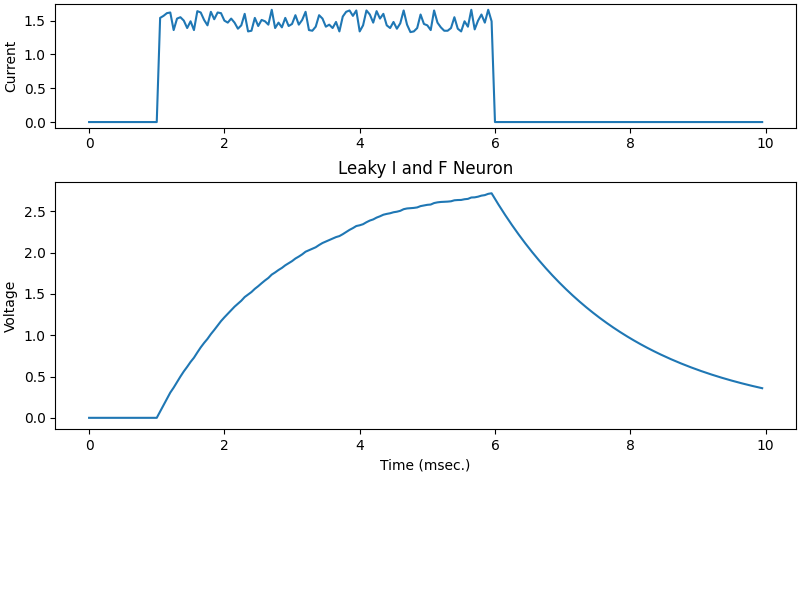
\includegraphics{LIF_plot.png}}
	
	\end{center}
	\caption{Example of a Leaky Integrate and Fire Neuron being injected with a current {i}}
\end{figure}

The Integrate and Fire model, IAF, shows how the membrane potential of a neuron reacts to an injection of current. If the membrane potential is injected with a high enough current it starts an all-or-nothing reaction resulting in a spike or action potential. The difference between the IAF model and the leaky integrate and fire model, LIF, is the existence of a reset mechanism in the LIF. Just like in the IAF model, when the LIF neuron reaches the threshold it fires and causes a spike. However, the leaky model can reset the membrane potential's voltage by using the reset by subtraction method. The reset by subtraction method is biologically more accurate because for real neurons, after firing, the neuron needs a higher voltage value to fire again.



% \subsection{Implementation of Membrane Potentials}

% In order to imitate behaviour of a neuron, SNNs have to keep and encode the membrane potential information. This is important, because membrane potential at the time  dictates to the neuron if it should fire, do nothing or enter refractory period. Membrane potential in SNNs can be expressed with the following equation:


% \begin{equation}
% 	V_{mem, j}^1(t) = V_{mem, j}^1(t-1) + z_j^l{t} - V_{th}\theta_j^l(t)
% \end{equation}

% \begingroup
% \fontsize{7pt}{9pt}\selectfont
% \begin{enumerate}
%     \item[] \begin{center}  $V_{mem, j}^1(t-1)$ = membrane potential at the previous time step, \end{center}
% 	\item[]  \begin{center} $z_j^l{t}$ is a sum of bias and products of weight and spikes, \end{center}
% 	\item[] \begin{center}  $V_{mem}$ = membrane voltage, \end{center}
% 	\item[] \begin{center}  $\theta_j^l(t)$ is a spike, \end{center}
% 	\item[] \begin{center}  $V_{th}$ = threshold voltage value. \end{center}
% \end{enumerate}
% \endgroup

Requirement to pass this information from layer to layer is one of the reasons why it is difficult to train Spiking Neural Networks (\citeA{kim2020spiking}). 

\section{Problems with Spiking Neural Networks}

\subsection{Loss of Information}

When a neuron in Spiking Network is either under- or over- activated, there might occur information loss. These events happen due to the input voltage being either too large and generating spikes regardless of the value of input or due to input voltage being too low and taking a long time to produce a spike. To solve these problems multiple normalization methods have been invented.

For example, \citeA{kim2020spiking} proposed a channel-wise data-based normalization that normalizes the weights bt the maximum possible activation in a channel-wise manner as opposed to a conventional layer-wise method. 

\subsection{Non-differentiability}

The issue with the SNN is that the spike events are non-linear, discrete events, which means that the rate of change, the derivative, is zero everywhere apart from when the value of the membrane potential is equal to zero (\citeA{surrogateGradient}). Thus, the SNN model can not use standard error backpropagation.

Alleviating the issue of the SNN model’s being non-differentiability in addition to optimizing the algorithm itself required either smoothing the SNN by making it continuously differentiable or introducing the surrogate gradient (SG) which is a “continuous relaxation of the real gradients” (\citeA{surrogateGradient}). snnTorch solves the non-differentiability issue for us by providing a custom backpropagation method that integradtes surrogate gradient. 

\subsection{Biological Icarus}

Just like in the story of Icarus and his father, creators of Spiking Neural Networks are trying to get close to biologically plausible neural network model while trying to not \textit{"melt their wings"} and fail. Due to this constraint, LIF seems to be the best candidate to simulate neurons without getting into too much biological detail.

All the challenges of implementation of Spiking Neural Networks that we mentioned before are the reason why standard Artificial Neural Networks rely on utility focused tools for achieving their goals. Indeed, introduction of more biologically plausible models are faced with problems when attempted to be implemented in code. This is the case with Leaky-Integrate-and-Fire and the reason why despite being the most biologically accurate, the Hodgkin's and Huxley's neuron model (H-and-H) is not likely to be used in AI and development of neural networks. Moreover, if someone would try to attempt a neural network with H-and-H model at the heart they would probably \textit{"get too close to the sun"} and fall.
\section{The Dataset}

For purposes of the project, we have chosen to use the Microsoft Common Objects in Context, a dataset of over 330 thousand images, with over 200 of these labeled, 80 categories of instances, and over 1.5 million object instances all together (\citeA{COCOdataset}). This substantial dataset is utilized with an API developed specifically to access the contents of the dataset, both of which have been made open-source by their developers \href{https://github.com/cocodataset/cocoapi}{(Link to the API)}. The objectives of MSCOCO are to detect and categorize objects found within images based on their iconicity, their position in relation to other objects, and the binding coordinates of space they occupy in a given image. 


\subsection{Properties of Data}
Notably, MSCOCO is proposed by its developers to be more effective at training object recognition models than other popular datasets that are used in research and the industry. These advantages of MSCOCO mainly lay in the following properties of the data and the dateset.


\begin{enumerate}
    \item Detecting non-iconic views \begin{itemize}
        \item In line with its focus of detecting images in their natural contexts, MSCOCO is designed to be more effective in detecting objects in non-iconic views than other datasets. When speaking to what iconicity means in this context, we mean a recognition system’s ability to interpret objects from an image, even when those objects are obscured by clutter, and layered deep behind occlusions which move them away from the image’s center-focus.
        \item On average, MSCOCO’s objects are smaller when compared to the sizes found in other popular datasets such as ImageNet and PASCAL, a feature which speaks to its greater efficiency at parsing through ambiguity and noise to detect the intended objects.
        \end{itemize}
    \item Contextual Reasoning
        \begin{itemize}
            \item MSCOCO also uses contextual reasoning where multiple objects are present, which demonstrates the improved ability to recognize them even when objects are not isolated, and are instead present amongst others. For instance, where previous datasets, such as ImageNet and PASCAL, account for 60\% of their images being object-isolated (meaning only depict a singular object), MSCOCO account for only 10\%. The processing of such contextually-ambiguous scenes further builds onto the dataset’s ability to object-recognize in natural scenes, and not just scenes where the object of interest is centrally-focused. 
        \end{itemize} 
    \item Object localization
        \begin{itemize}
            \item Given the effort MSCOCO places on contextual reasoning, and the importance of parsing through non-iconic scenes, it’s important to also understand that (a) MSCOCO requires, and indeed has, the ability of object localization–that is, the ability to process the spatial relations between objects in a scene; and (b), how MSCOCO segments this object localization.
        \end{itemize}
\end{enumerate}

\subsection{Functionality of Data}

When observed, the dataset can first be categorized by the type of objects being analyzed, and secondly by what object of the category is being analyzed. 

Of the 80 categories offered, we focus on 10, which can be classified as animals: bird, cat, dog, horse, sheep, cow, elephant, bear, zebra, and giraffe. Using this dataset, we aim to train a spiking neural network to demonstrate the intended object-recognition model.

Functionally, when an image is analyzed, the program identifies key attributes which are used to categorize appropriately. For instance, where we analyze an image of two giraffes, we should consider the properties of the data used in the process of segmentation.

\begin{figure}[h]
	\begin{center}
		\scalebox{0.4}{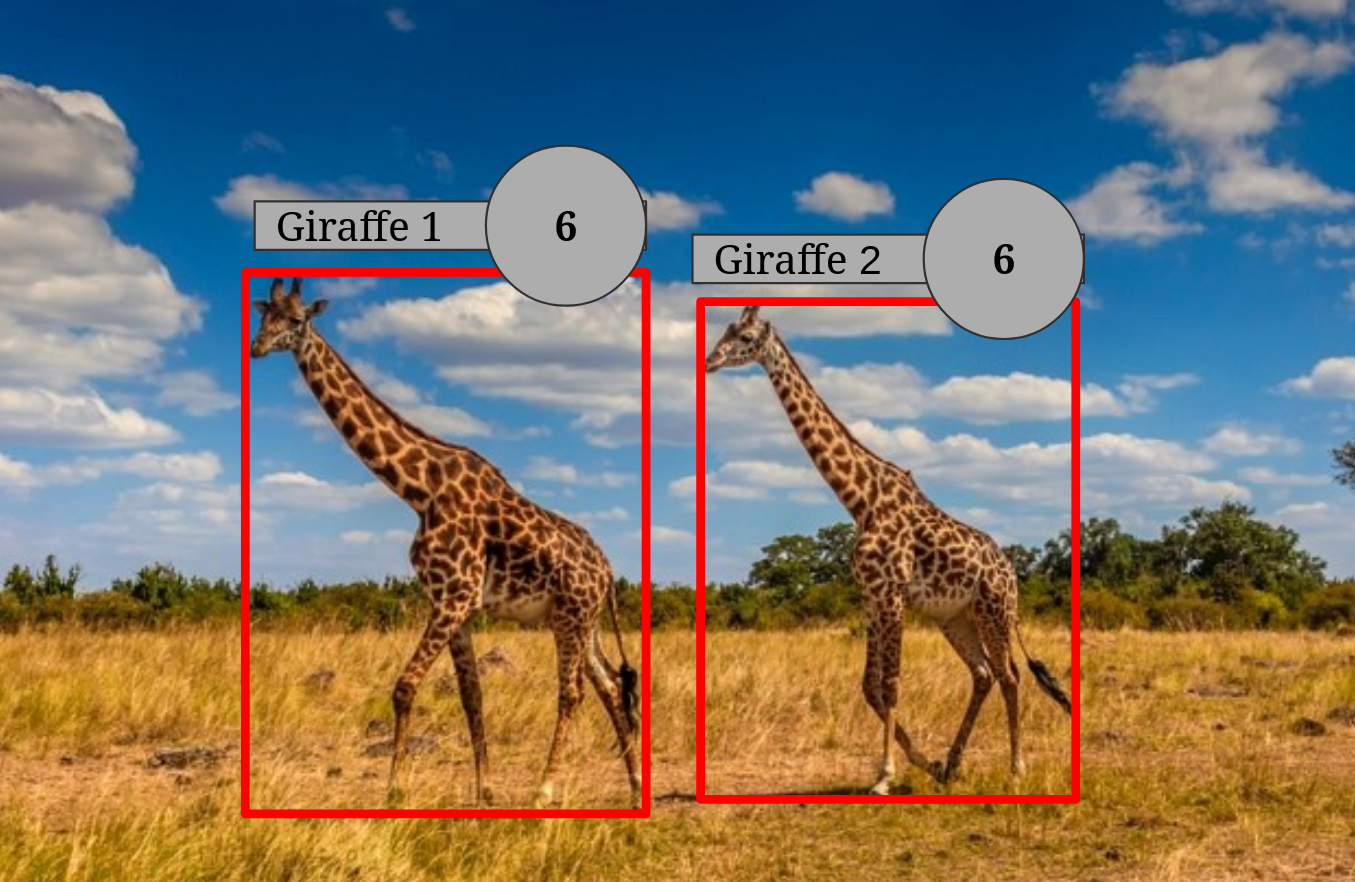
\includegraphics{giraffe.png}}
	
	\end{center}
	\caption{Example of an image from the MSCOCO dataset with the annotations that it contains.}
\end{figure}

\begin{enumerate}
    \item Boxes 
        \begin{itemize}
        \item The image presented is first identified by a “bounding box”; this box is important for object localization. It provides the minimum and maximum coordinates along a cartesian-plane to identify the boundaries of space an object occupies.
        \end{itemize}
    \item Area
        \begin{itemize}
            \item Within the bounding box, a pixel count for each object present is processed and utilized to further understand the iconicity and/or ambiguity of the object in relation to its scene.
        \end{itemize} 
    \item Label
        \begin{itemize}
            \item This property output can be read to distinguish (a) the number of object-instances found in an image, and (b) the category each object-instance.
        \end{itemize}
\end{enumerate}


\begin{wrapfigure}[25]{r}{0.42\textwidth}
	\begin{center}
		\scalebox{0.45}{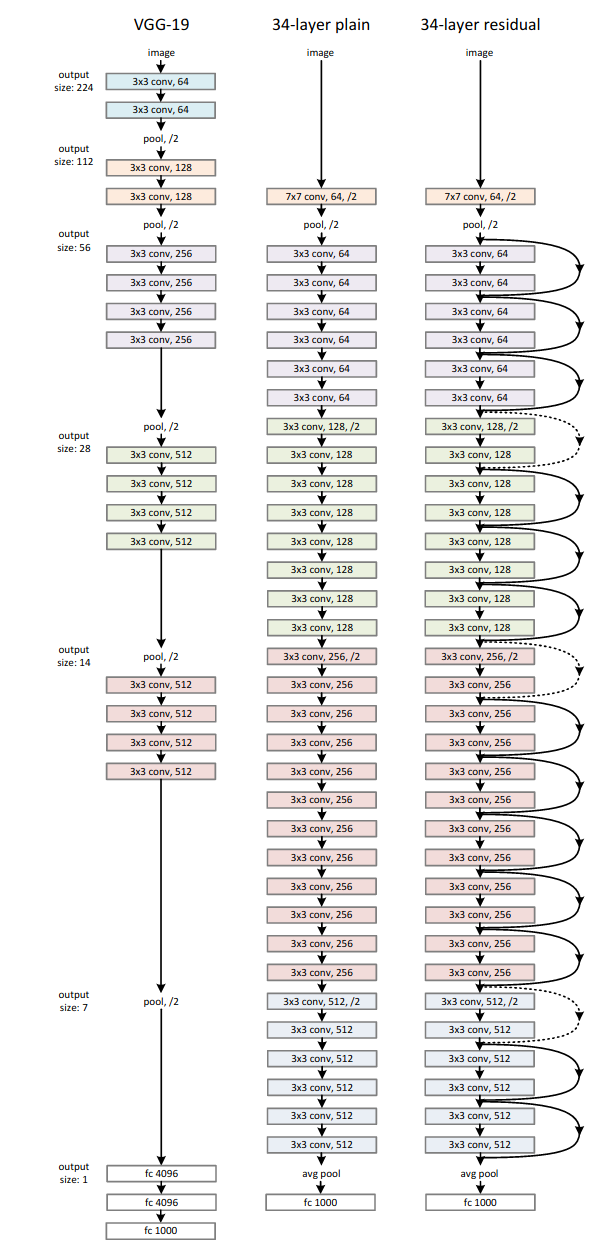
\includegraphics{resnet_comp.png}}
	\end{center}
		\caption{Examples of 16-layer VGG, Plain 34-layer, and 34-layer ResNet Network 
		Architectures}
\end{wrapfigure}

The described properties of the image annotation should be considered in relation to the process segmentation in object recognition. Mainly, it’s important to consider that object-segmentation is a difficult process and requires an accurate bounding boxes prediction. Furthermore, considering that the dataset holds over 1.5 million category instances, given the sheer magnitude and complexity of the dataset efficiency plays a big role in training a neural-network that utilizes this dataset. As such, a major goal of our assignment is to build and train a spiking neural network model to do so.  


\section{Architectures Of Deep Neural Networks}

When it comes to building a neural network, one has to establish an
architecture or an arrangement of layers and how they connect with each other.
It is particularly important, when the network increases in complexity. Object
classification + localization being a demanding task for a network to solve,
we have adopted a published and well-tested architecture for the task --
ResNet. The particular architecture we have tried to imitate titled 
\textit{DECOLLE}, was first developed by \citeA{kaiser2018synaptic} and later
enhanced by \citeA{barchid2021deep}. \textit{DECOLLE} Neural Network adopts 
properties of classical ResNet model architecture as well as a pyramidal structure that
was proposed by \citeA{pyramid}. 

\subsection{ResNets}

\begin{wrapfigure}[21]{r}{0.42\textwidth}
\begin{center}
	\scalebox{0.35}{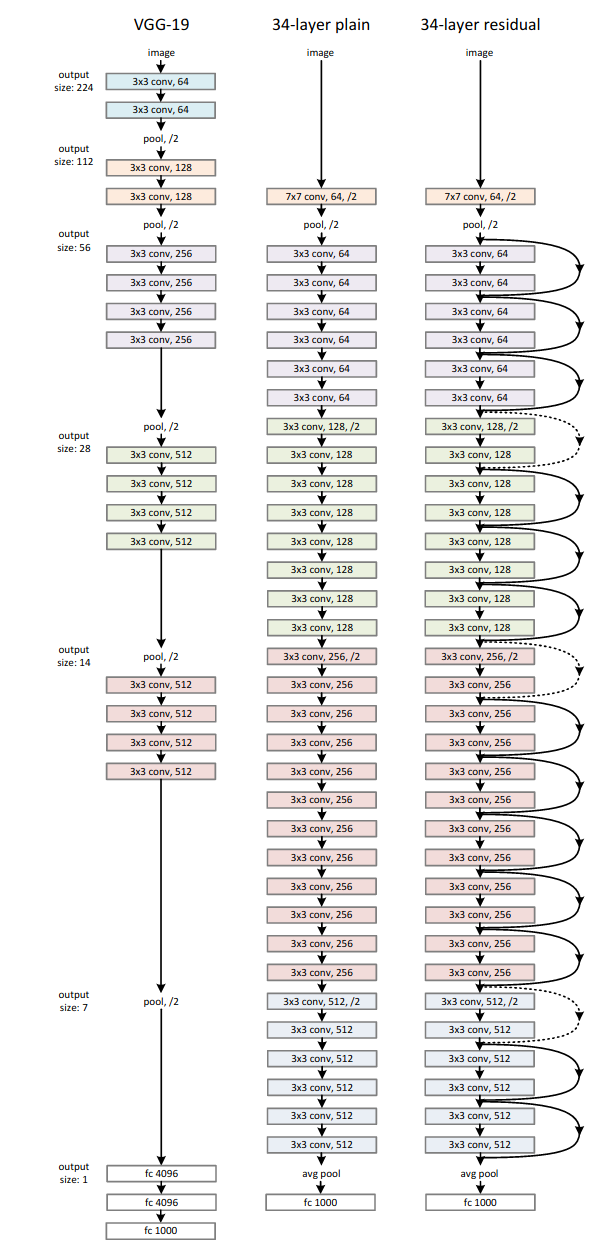
\includegraphics{resnet_comp.png}}
\end{center}
	\caption{Examples of 16-layer VGG, Plain 34-layer, and 34-layer ResNet Network 
	Architectures}
\end{wrapfigure}




To begin with the cornerstone of our architecture -- ResNet, it was named for its property,
of convolutional layers of the network that are residually connected with each other using
shortcut connections (\citeA{resnet}).
According to the authors of the original paper on ResNets,
addition of residual connections improves model's convergence, or ability for
model's loss to move towards a minimum with a decreasing trend. Meanwhile,
ResNets converge faster than their plain counterparts, the complexity of 
ResNets is much lower than complexity of well established Visual Geometry
Group (VGG) Networks given the same depth (3.6 billion FLOPs (Float Point 
Operations) vs. 19.6 billion FLOPs) (\citeA{resnet}). 

\subsection{Comparing Model Performance}
To compare networks' performance one has to understand how it is measured and what
constitutes an accurate model. For the task of object detection/localization accuracy
of the model at predicting class of the object in the image is not enough. Thus,
two additional performance metrics have been adapted : Mean Average Precision (mAP) and
Intersection of Union (IoU). Firstly, Mean Average Precision for the purposes of Object
Detection is well-defined in the paper by \citeA{evaluation}. According to the authors,
mAP is mean of Average Precision of the model for all the classes in the dataset. It is
calculated using the following equation.


\begin{equation}
	\textbf{mAP} = \frac{1}{N} * \sum_{i = 1}^{N} \textbf{AP}_i
\end{equation}

\begingroup
\fontsize{7pt}{9pt}\selectfont
\begin{enumerate}
	\item[]  \begin{center} AP = Average Precision, \end{center}
	\item[] \begin{center}  N = number of classes. \end{center}
\end{enumerate}
\endgroup


Next, IoU is the area of overlap of ground-truth boxes and the model's detected box output,
the higher the IoU the better performance of the model. Intersection of Union can be 
represented as follows:

\begin{equation}
	\textbf{IoU} = |A \cap B| \div  |A \cup B| = |I| \div |U|
\end{equation}

\begingroup
\fontsize{7pt}{9pt}\selectfont
\begin{enumerate}
	\item[]  \begin{center} I = Intersection area, \end{center}
	\item[] \begin{center}  U = Union area. \end{center}
\end{enumerate}
\endgroup


\subsection{Pyramidal Architecture of Neural Network}


Pyramidal structure of a Neural Network refers to the shape of the layers as the model
gets deeper. With each layer dimensions of convolutional layers shrink (usually in half).
For example, the first convolutional layer would have input dimension equal to number of
channels in the image (3 channels in case of RGB images vs. 1 for grayscale) and the output
dimension of 512, with next layer input equal to previous layer's output. Second layer
would have the dimension of 256 (half of previous layer's output) and so on (\citeA{pyramid}).

For the purposes of our network, pyramidal structure of neural network is leveraged using
Encoder-Decoder model. When image is passed through the shrinking layers of the Encoder
Pyramid, it loses resolution as well as contextual information, however when the image
leaves the encoder and is located in the hidden state it is fully comprised of
the semantic information about the image (What object is on the picture and where it is
located). Furthermore, in order to localize an object on the image that model has never 
encountered before, it has to be able to place the semantic information in context. 
This is where Decoder comes into play, being the reverse of an Encoder, the convolutional
layers of decoder double in size until desired dimensions. The decoder is residually
connected to encoder, and thus it gains contextual information about the image through
every pass of a layer.

At the end, in order to extract meaningful, last decoder layer is connected
to fully connected linear layers that  output predicted class as well as
detected box coordinates.





\subsection{Architecture of the Model Used}


Architecture developed by \citeA{barchid2021deep} was the target to replicate. The model is based
on Encoder-Decoder architecture with residually connected layers akin to ResNets. Encoder and 
Decoder follow the pyramidal architecture that was discussed earlier. 

\begin{figure}[h]
	\begin{center}
		\scalebox{0.4}{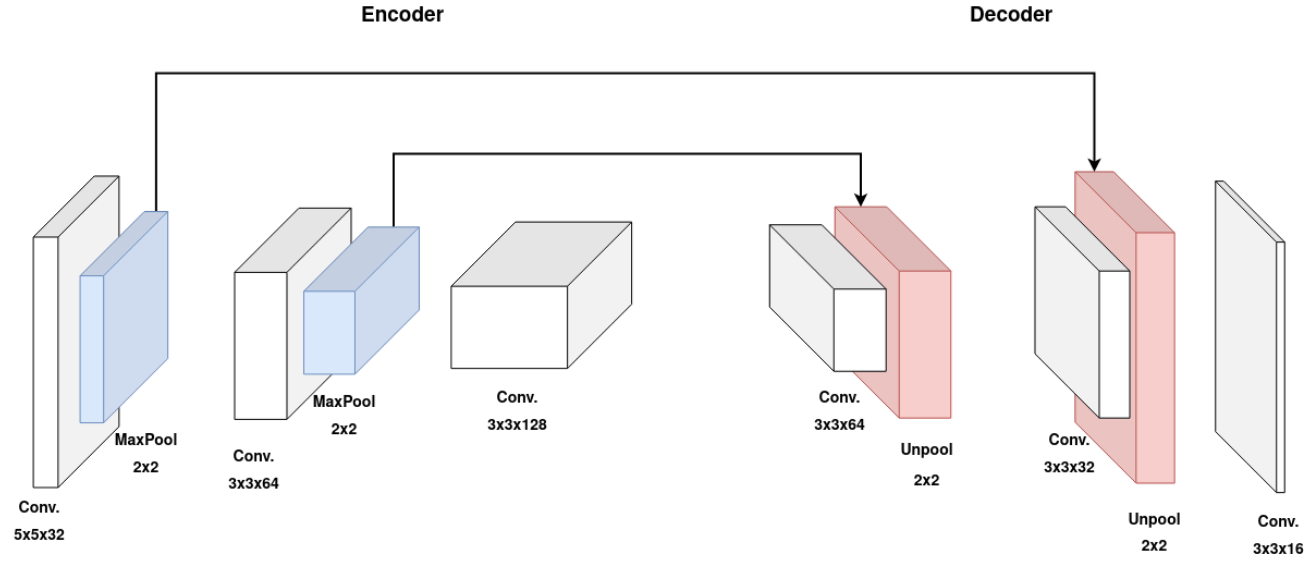
\includegraphics{barchid_SED.png}}
	
	\end{center}
	\caption{Sketch of the model's architecture. White layers represent convolutional layers,
	blue represent pooling layers, and red unpooling layers}
\end{figure}




\section{Implementation}

\subsection{PyTorch}

The main package that allowed us to develop such a complex model was PyTorch. PyTorch
is an open-source a machine learning/deep learning library and framework for Python 
that allows user to develop and ship high performance models (\citeA{pytorch}). This library
eliminates the need from scratch development of the most important methods in machine learning,
such as activation functions, model architecture assembly, 


\subsection{Spiking Neurons}

Given the complexity of Spiking Neural Networks and the integration of Leaky-Integrate-and-Fire
into the network, we used a package that allows to use LIF within a PyTorch model -- 
\href{https://snntorch.readthedocs.io/en/latest/snntorch.html}{\textit{snnTorch}}. 
snnTorch also allowed us to integrate backpropogation for spiking neural networks
with one line. Indeed, to use LIF in your model only need to use one line in model
definition.

\begin{lstlisting}[language=Python, caption=Leaky-Integrate-and-Fire using snnTorch]
	import snntorch as snn
	spike_grad = surrogate.fast_sigmoid(slope=25)
	beta = 0.5

	lif1 = snn.Leaky(beta=beta, spike_grad=spike_grad)

\end{lstlisting}

\section{Challenges}

With the number of operations required to train the model to complete the task of object
localization, it was clear since the beginning that a lot of compute power was required. A number
of steps was required in order to make this project plausible the scope of this course.

First challenge in implementation of the model was difficulty to replicate the 
\citeA{barchid2021deep} paper given how the lack of description on the implimintation in the 
paper as well non-existence of public repository with the code for their model.



\newpage
\bibliographystyle{apacite}

\bibliography{report}

\end{document}